\documentclass[a4paper,12pt]{article}
\usepackage[spanish]{babel}
\hyphenation{co-rres-pon-dien-te}
%\usepackage[latin1]{inputenc}
\usepackage[utf8]{inputenc}
\usepackage[T1]{fontenc}
\usepackage{graphicx}
\usepackage[pdftex,colorlinks=true, pdfstartview=FitH, linkcolor=blue,
citecolor=blue, urlcolor=blue, pdfpagemode=UseOutlines, pdfauthor={H. Asorey},
pdftitle={Física 1A - Guía 02}]{hyperref}
\usepackage[adobe-utopia]{mathdesign}

\hoffset -1.23cm
\textwidth 16.5cm
\voffset -2.0cm
\textheight 25.8cm

%----------------------------------------------------------------
\begin{document}
\title{
{\normalsize{Universidad Nacional de Río Negro - Profesorados de Física y
Química}}\\
Física I A \\ Guía 02 - Energía}
\author{Asorey - Cutsaimanis}
\date{2016}
\maketitle

\begin{enumerate}

\item {\bf{Cuentas}}

Repase, rehaga y verifique todas las cuentas y cálculos parciales realizados en
clase.

\item {\bf{Energía potencial gravitatoria}}

\begin{enumerate}
\item La energía potencial gravitatoria entre dos cuerpos de masas $m_1$ y $m_2$
separados por una distancia $r$ está dada por: 
\[
E_g = -\frac{G m_1 m_2}{r}.
\]
De esta forma, la energía potencial gravitatoria de un cuerpo de masa $m$ sobre
la superficie de un planeta de masa $M$ y radio $R$ es: 
\[
E_g = -\frac{G M m}{R}.
\]
Verifique que al elevar ese cuerpo a una altura $h$ sobre la superficie del
planeta, la variación de la energía potencial gravitatoria es: 
\[
\Delta E_g = G M m \left ( \frac{1}{R} - \frac{1}{R+h} \right ).
\]
\item Calcule la energía potencial para un astronauta ($m=70$\,kg) en órbita a
una altura $h=350$\,km. Luego, compare ese valor con el obtenido de la expresión 
aproximada $\Delta E_g = m g h$.
\end{enumerate} 

\item{\bf{Esquiadores}}.

Se prepara una pista en el cerro Catedral a $h_i=2400$\,m\,s.n.m. alisada para
pista de bajada hasta la base ($h_f=1030$\,m\,s.n.m) Un esquiador se propone
superar el récord mundial, actualmente de $251.4$\,km\,h$^{-1}$. Usando
argumentos de conservación de la energía, y despreciando todo efecto de
rozamiento, diga si esto es posible, y calcule cuál es la velocidad máxima que
podría alcanzarse. ¿Depende de la masa del esquiador? Justifique.

\item{\bf{Fútbol}}.

Un nene que vive en el último piso del Bariloche Center ($h=30$\,m) se va a jugar al
fútbol. Al llegar a la planta baja se da cuenta que no trajo su pelota ($m=400$\,g). 
Llama por celular a su padre para que le arroje la pelota por la ventana.
\begin{enumerate}
\item ¿Cuál es la variación de la energía potencial entre el techo y la base
del edificio?
\item Determine la variación de la energía cinética y la velocidad de la pelota
cuando esta llega al piso.
\end{enumerate}

\item {\bf{Impacto}}.

La extinción de los dinosaurios al final del período Jurásico es atribuida al
impacto de un cometa o meteorito de dimensiones considerables. Imagine entonces
que un cometa esférico de radio $r=5$\,km y densidad media $d=5$\,g\,cm$^{-3}$
se acerca a la Tierra desde el infinito. Entonces,

\begin{enumerate}
\item Calcule la masa $m_c$ del cometa.
\item Calcule la energía cinética y la velocidad al momento del impacto.
\item Exprese la energía liberada en el impacto en megatones, teniendo en cuenta
que $1$\,Mton $= 4.184 \times 10^{15}$\,J.
\item Si debido a la interacción atmosférica el satélite se divide en dos partes
de masas $m_1=0.7 m_c$ y $m_2=0.3 m_c$. Calcule la energía cinética y la
velocidad de cada parte al momento del impacto. ¿Dependerá el resultado de la
altura a la cual el cometa se parta? Justifique.
\end{enumerate}

\item {\bf{Rebotes}}.

Una pelota de goma de masa $m=2.0$\,kg es lanzada hacia arriba en forma
vertical. La velocidad inicial es de $v=5$\,m s$^{-1}$.
\begin{enumerate}
\item Calcule la altura máxima que alcanza la pelota en su trayectoria;
\item suponiendo que no hay pérdidas de energía debidas al rozamiento, calcule
la velocidad al momento del impacto y la altura alcanzada luego del rebote.
\item Suponga que, a diferencia del punto anterior, como consecuencia del
rebote un $20\%$ de la energía mecánica se transforma en calor y sonido.
Calcule la altura que alcanzará la pelota luego de tres choques contra el piso.
\end{enumerate}

\item{\bf{Resortes}}

La energía potencial elástica está dada por:
\[E_e = \frac{1}{2} k (\Delta x)^2 \]
donde $k$ es la constante elástica del resorte y $\Delta x$ representa a la
variación de la longitud del resorte en condiciones de compresión o expansión.
Imagine entonces que usted debe diseñar el sistema de protección de resortes de
un ascensor en el Bariloche Center ($h=30.0$\,m), y que los mismos pueden
comprimirse un máximo de $0.5$\,m. Sabiendo que la masa del ascensor y su carga
es de $m=600$\,kg, 

\begin{enumerate}
\item calcule la constante $k$ del resorte;
\item si el ascensor tiene un freno de seguridad capaz de transformar el $20\%$ de
la energía cinética, calcule el $k$ del resorte necesario en este caso;
\item Rehaga los cálculos anteriores pero suponiendo que en lugar de un único
gran resorte se disponen cuatro resortes más pequeños. 
\end{enumerate}

\item {\bf{Pesos}}.

A partir de la definición de $g$, 
\[
g=\frac{GM}{R^2},
\]
para un cuerpo esférico de masa $M$ y radio $R$, 
\begin{enumerate}
\item calcule el valor de $g$ y determine cuál es el peso de un cuerpo de masa
$m=70$\,kg en la Tierra, el Sol, Júpiter y la Luna; 
\item calcule a que altura $h$ sobre la superficie de la Tierra, un cuerpo pesa la mitad respecto a su peso sobre la superficie terrestre. 
\item ¿Qué pasaría si realizamos el mismo cálculo en el planeta Marte?
\end{enumerate}

\item {\bf{Velocidad de escape}}

Se define como {\emph{velocidad de escape}} a aquella velocidad $v_c$ para la
cual un cuerpo de masa $m$ (cuerpo A) puede escapar de la atracción gravitatoria
de otro cuerpo (cuerpo B).

Imaginemos que el cuerpo B es un planeta de radio $R$ y masa $M$, y colocamos al
cuerpo A sobre su superficie. Entonces,
 
\begin{enumerate}
\item Obtenga una expresión para el cálculo de la velocidad de escape, y
muestre que la misma es una propiedad inherente del planeta.
\item Grafique la dependencia de la velocidad de escape como función:
\begin{itemize}
\item del radio $R$ del planeta.
\item de la masa $M$ del planeta.
\end{itemize}
\item Calcule el valor de la velocidad de escape sobre la superficie de 
\begin{enumerate}
\item la Tierra
\item la Luna
\item el Sol 
\item una pelota de fútbol de radio $R=12.5$\,cm y $m=0.4$\,kg 
\end{enumerate}
\item Suponga que es posible variar a voluntad el radio terrestre $R_\oplus$.
Calcule el valor de $R_\oplus \equiv R_c$ para el cual la velocidad de escape
de la Tierra sea igual a la velocidad de la luz $c$.
\item Libere su imaginación y responda: ?`Qué pasaría si, una vez alcanzado
dicho radio crítico, aumentamos la masa de la Tierra?
\end{enumerate}

\item {\bf{El Principito}}

El Principito ($m=40$\,kg) vive en un planeta pequeño, el asteroide B612.
Supongamos que posee un radio $R = 1$\,km con una densidad igual a la de la
Tierra ($d = 5.5$\,g\,cm$^{-3}$). Calcule
\begin{enumerate}
\item el valor de $g$ y el peso del Principito en B612;
\item si en la Tierra el Principito logra subir a una silla de $h=0.5$\,m de un
salto, a que altura llegará con el mismo salto sobre la superficie de B612.
\item la velocidad máxima a la cual el Principito puede caminar sin riesgo de
abandonar el planeta para siempre
\end{enumerate}
\end{enumerate}
\centering 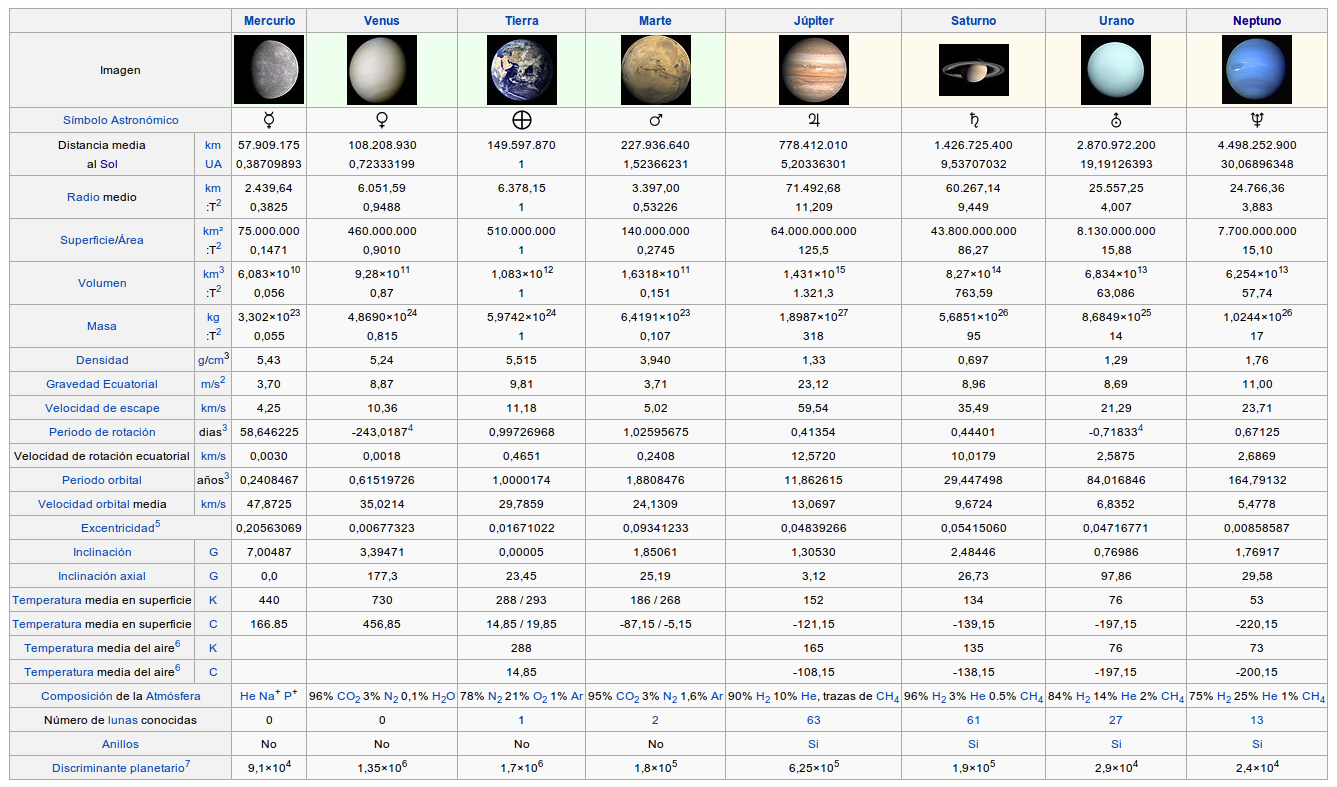
\includegraphics[angle=90,width=0.95\textwidth]{planetas.png}

\end{document}
%%%%
